\begin{frame}{Kiến trúc Agentic RAG bằng LangGraph}
\begin{figure}[H]
\centering
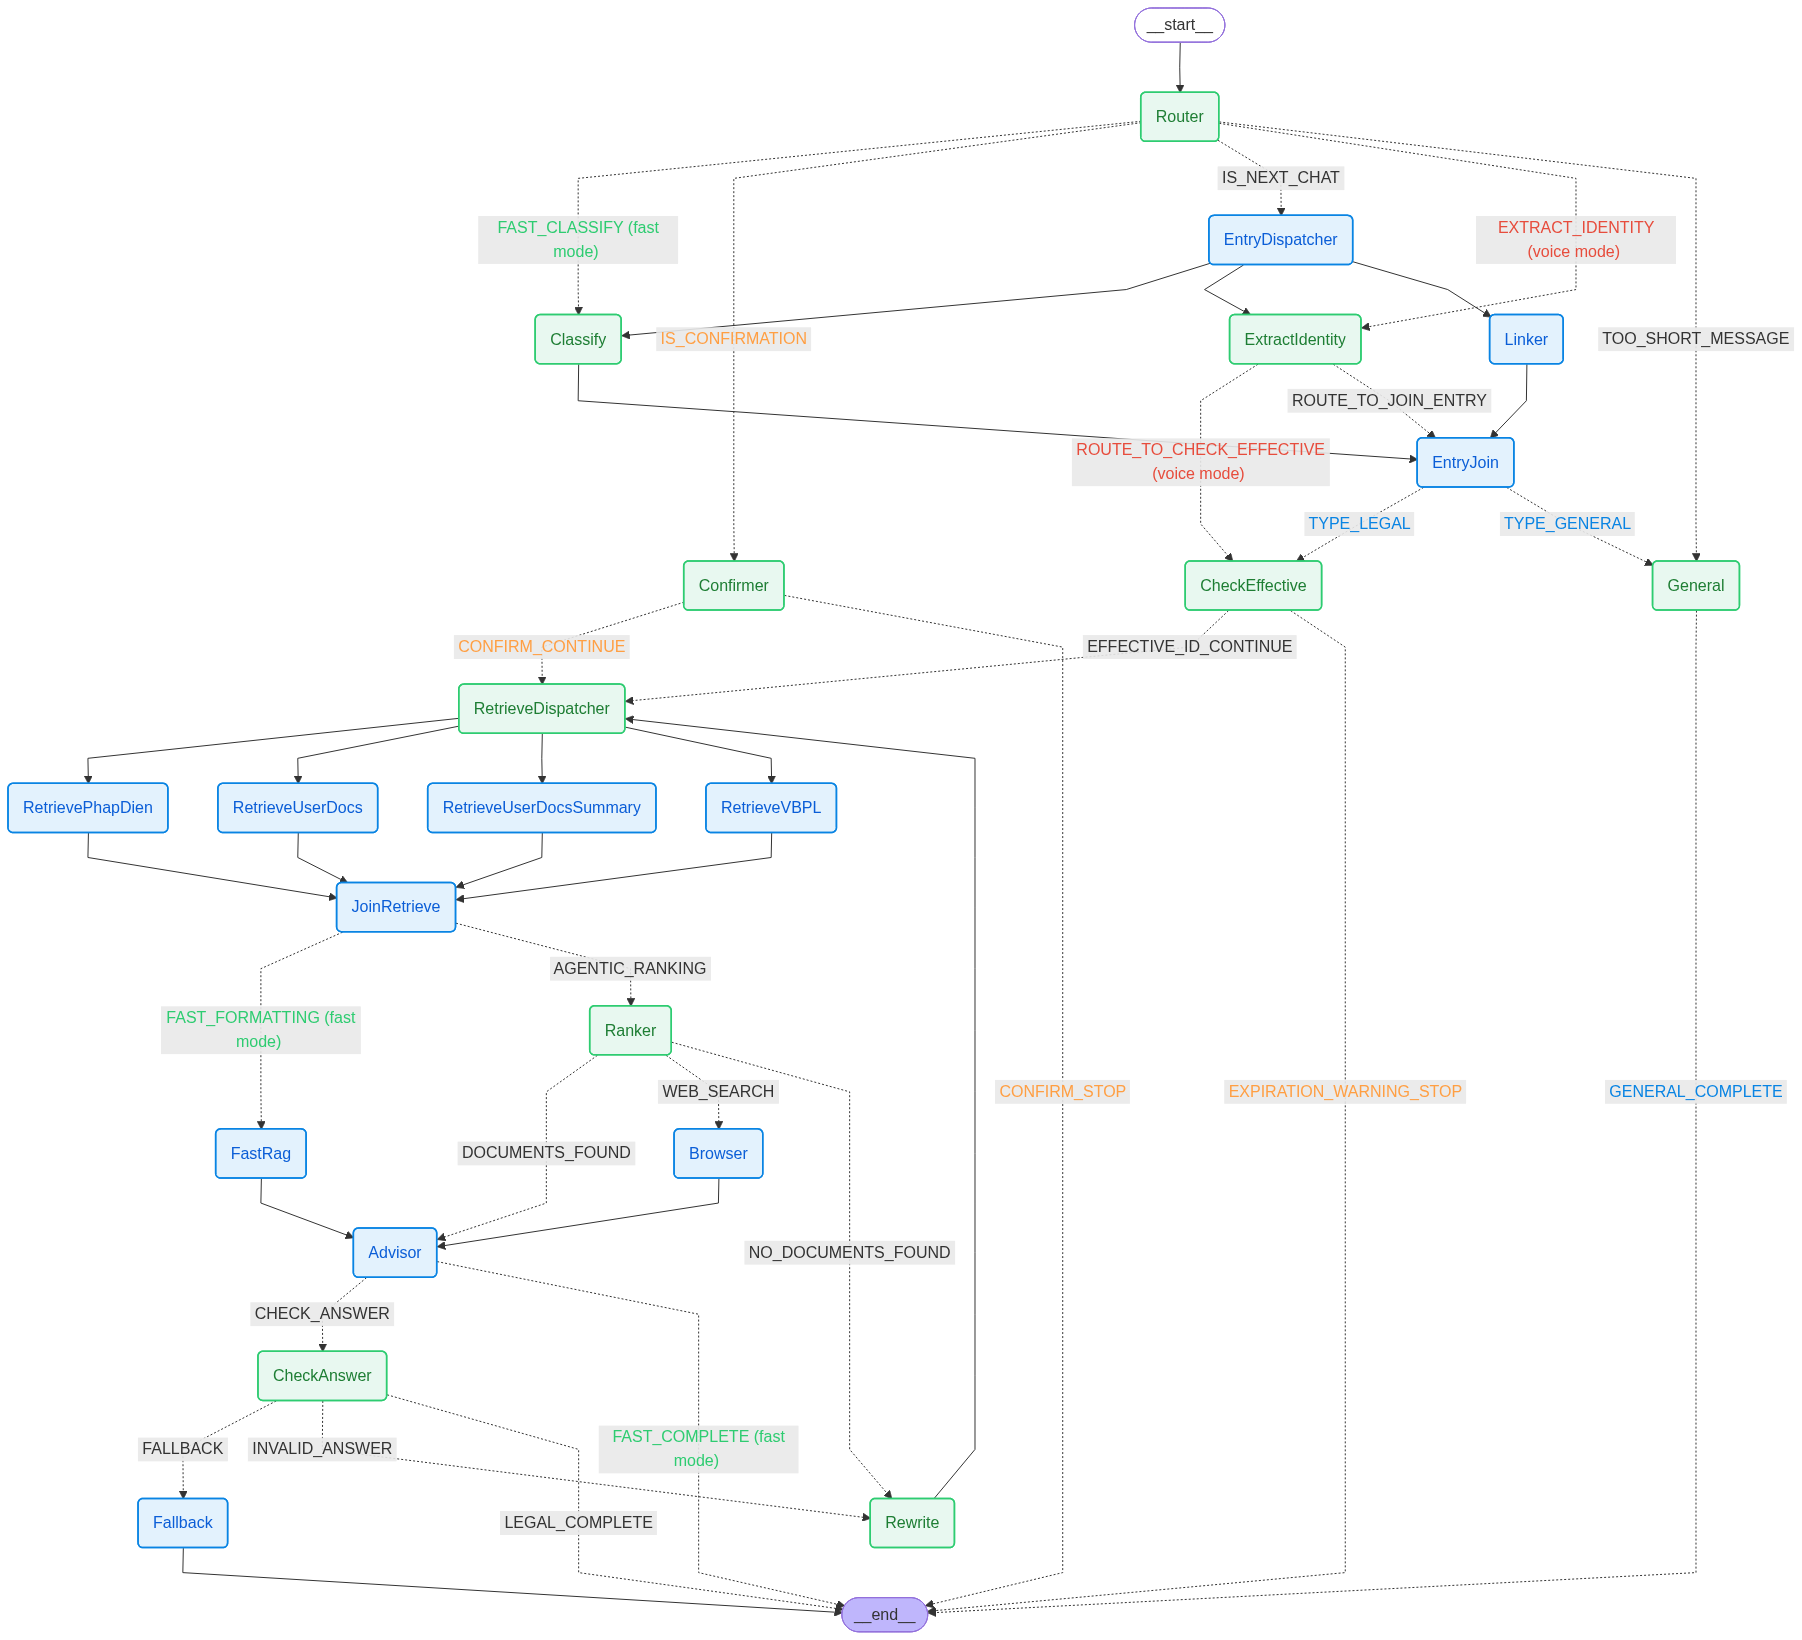
\includegraphics[height=0.55\textheight,width=0.9\textwidth,keepaspectratio]{pictures/rag_diagram.png}
\caption{Sơ đồ LangGraph của dự án}
\end{figure}

\note{
Đây là sơ đồ Agentic RAG của dự án được xây dựng bằng LangGraph. Hệ thống phân chia thông minh giữa mô hình nhỏ cho luồng cơ bản (màu xanh lá) và mô hình lớn cho các tác vụ suy luận phức tạp (màu xanh dương) để tối ưu chi phí và độ trễ.
Mỗi tin nhắn đi qua Router để kiểm tra điều kiện và định tuyến qua các node như rewrite query, retrieve tài liệu và sinh câu trả lời.
}
\end{frame}
